\documentclass[12pt]{article}
\usepackage{url}
\usepackage[hidelinks]{hyperref}
\usepackage{graphicx}
\usepackage{caption}
\usepackage[export]{adjustbox}
\usepackage{setspace}
\usepackage{wrapfig}
%\usepackage[utf8]{inputenc} %utf8 % lettere accentate da tastiera
\usepackage[italian]{babel} % lingua del documento
% \usepackage{dirtree}
% \usepackage{caption}
% \usepackage{subcaption}
\usepackage{listings}

\usepackage{listings}
\usepackage{xcolor}

\colorlet{punct}{red!60!black}
\definecolor{background}{HTML}{EEEEEE}
\definecolor{delim}{RGB}{20,105,176}
\colorlet{numb}{magenta!60!black}

\definecolor{Code}{rgb}{0,0,0} 
\definecolor{Decorators}{rgb}{0.5,0.5,0.5} 
\definecolor{Numbers}{rgb}{0.5,0,0} 
\definecolor{MatchingBrackets}{rgb}{0.25,0.5,0.5} 
\definecolor{Keywords}{rgb}{0,0,1} 
\definecolor{self}{rgb}{0,0,0} 
\definecolor{Strings}{rgb}{0,0.63,0} 
\definecolor{Comments}{rgb}{0,0.63,1} 
\definecolor{Backquotes}{rgb}{0,0,0} 
\definecolor{Classname}{rgb}{0,0,0} 
\definecolor{FunctionName}{rgb}{0,0,0} 
\definecolor{Operators}{rgb}{0,0,0} 
\definecolor{Background}{rgb}{0.98,0.98,0.98} 

\lstdefinelanguage{json}{
    basicstyle=\normalfont\ttfamily,
    numbers=left,
    numberstyle=\scriptsize,
    stepnumber=1,
    numbersep=8pt,
    showstringspaces=false,
    breaklines=true,
    frame=lines,
    backgroundcolor=\color{background},
    literate=
     *{0}{{{\color{numb}0}}}{1}
      {1}{{{\color{numb}1}}}{1}
      {2}{{{\color{numb}2}}}{1}
      {3}{{{\color{numb}3}}}{1}
      {4}{{{\color{numb}4}}}{1}
      {5}{{{\color{numb}5}}}{1}
      {6}{{{\color{numb}6}}}{1}
      {7}{{{\color{numb}7}}}{1}
      {8}{{{\color{numb}8}}}{1}
      {9}{{{\color{numb}9}}}{1}
      {:}{{{\color{punct}{:}}}}{1}
      {,}{{{\color{punct}{,}}}}{1}
      {\{}{{{\color{delim}{\{}}}}{1}
      {\}}{{{\color{delim}{\}}}}}{1}
      {[}{{{\color{delim}{[}}}}{1}
      {]}{{{\color{delim}{]}}}}{1},
}



 
\lstdefinelanguage{Python}{ 
numbers=left, 
numberstyle=\footnotesize, 
numbersep=1em, 
xleftmargin=1em, 
framextopmargin=2em, 
framexbottommargin=2em, 
showspaces=false, 
showtabs=false, 
showstringspaces=false, 
frame=l, 
tabsize=4, 
% Basic 
basicstyle=\ttfamily\small\setstretch{1}, 
backgroundcolor=\color{Background}, 
% Comments 
commentstyle=\color{Comments}\slshape, 
% Strings 
stringstyle=\color{Strings}, 
morecomment=[s][\color{Strings}]{"""}{"""}, 
morecomment=[s][\color{Strings}]{'''}{'''}, 
% keywords 
morekeywords={import,from,class,def,for,while,if,is,in,elif,else,not,and,or,print,break,continue,return,True,False,None,access,as,,del,except,exec,finally,global,import,lambda,pass,print,raise,try,assert}, 
keywordstyle={\color{Keywords}\bfseries}, 
% additional keywords 
morekeywords={[2]@invariant,pylab,numpy,np,scipy}, 
keywordstyle={[2]\color{Decorators}\slshape}, 
emph={self}, 
emphstyle={\color{self}\slshape}, 
% 
} 


% \graphicspath{ {images/} }

\title{%
    Big Data Velocity\\
    \large Ottenimento e analisi di dati in streaming}

\begin{document}
\maketitle
\pagenumbering{roman}
\tableofcontents

\newpage
\pagenumbering{arabic}
\setcounter{page}{1}
\section{Introduzione}

Questo progetto nasce con l'obiettivo di ottenere dati in streaming e di sottoporli ad un'analisi
in tempo reale.\\
Il dominio scelto è quello finanziario, nello specifico quello delle criptovalute in quanto le piattaforme di exchange formiscono API di semplice accesso che consentono di ricevere informazioni di mercato come prezzi e volumi di un certo asset con tempi di ritardo ridotti.\\
In aggiunta le monete virtuali negli ultimi anni hanno guadagnato una notevole attenzione mediatica tanto che ad esempio su servizi come Twitter ogni minuto vengono pubblicate varie decine di tweets relativi all'argomento. Grazie alle API fornite da Twitter è possibile ricevere questi tweets in streaming così da poter utilizzare anch'essi per scopi analitici.
\section{Dati}

I dati acquisiti dall'applicazione in tempo reale sono di tipo \textbf{time-series} o serie
temporali; si tratta di dati strettamente dipendenti da una coordinata temporale (ad esempio
il momento di acquisizione) e che presentano come conseguenza alcune peculiarità come il fatto
che spesso sono i dati recenti ad essere più "interessanti" e di conseguenza raramente si ha
la necessità di aggiornare dati passati.
\\
Ne sono alcuni esempio i dati acquisiti da sensori ad esempio metereologici, quelli relativi
all'utilizza delle risorse hardware di un personal computer o quotazioni di titoli finanziari.

\subsection{Dati finanziari}

I dati finanziari sono ricevuti dalla piattaforma di exchange di criptovalute Binance \cite{binance}
e comprendono i migliori prezzi di offerta e richiesta di un determinato simbolo e le rispettive
quantità; segue un esempio:

\begin{lstlisting}[language=json,firstnumber=1]
{
    "u": 5828881697,        // order book updateId
    "s": "BTCUSDT",         // symbol
    "b": "10262.83000000",  // best bid price
    "B": "1.88008400",      // best bid qty
    "a": "10262.94000000",  // best ask price
    "A": "6.48000500"       // best ask qty
}
\end{lstlisting}
%
I dati sono forniti in real-time senza nessun parametro temporale; di conseguenza verrà
aggiunto al momento della ricezione un campo "timestamp" con l'istante corrente come valore.
Durante l'analisi verrà principalmente utilizzato il valore "askprice".

\subsection{Tweets}

Anche i tweets possono essere considerati serie temporali data la notevole importanza
dell'istante di pubblicazione, soprattuto se analizzati per legati alla finanza.
\\
Sono ricevuti attraverso le API per sviluppatori fornite da Twitter \cite{twitter} e si
presentano come segue:

\begin{lstlisting}[language=json,firstnumber=1]
{
    "created_at": "Wed Sep 09 15:19:42 +0000 2020",
    "id": 1303714706687963136,
    "id_str": "1303714706687963136",
    "text": "... $50 ETH GIVEAWAY ...",
    "source": "...",
    "truncated": false,
    "in_reply_to_status_id": null,
    "in_reply_to_status_id_str": null,
    "in_reply_to_user_id": null,
    "in_reply_to_user_id_str": null,
    "in_reply_to_screen_name": null,
    "user": {
        ...
    }
    "geo": null,
    "coordinates": null,
    "place": null,
    "contributors": null,
    "retweeted_status": {
        ...
    }
    "is_quote_status": false,
    "quote_count": 0,
    "reply_count": 0,
    "retweet_count": 0,
    "favorite_count": 0,
    "entities": {
        ...
    }
    "favorited": false,
    "retweeted": false,
    "possibly_sensitive": false,
    "filter_level": "low",
    "lang": "en",
    "timestamp_ms": "1599664782579"
}
\end{lstlisting}
%
Si nota la presenza di ben 2 campi temporali ("created\_at" e "timestamp\_ms") che
rappresentano in realtà il medesimo istante temporale ma con precisione differente.
Tuttavia è possibile notare un certo ritardo nella ricezione dei tweets di circa 5-10
secondi, perciò è risultato necessario un campo aggiuntivo chiamato "received\_at" così
da tenere traccia del momento di ricezione.
L'analisi verrà successivamente effettuata principalmente sul campo "text" contente il
corpo del tweet.

Lo schema di entrambe le categorie di dati è costante per ogni messaggio rendedoli dati
strutturati o semi-strutturati per quanto riguarda i tweets, che presentano uno schema più complicato contente
elementi innestati (abbreviati nell'esempio per motivi di spazio) e del testo.
Nonostante ciò, anche per il fatto che dell'intero tweet i campi analizzati saranno il testo
e le coordinate temporali, è possibile utilizzare una rappresentazione relazionale.

% 2 parole sul fatto che sono strutturati

% sono timeseries
\section{Componenti software}

Seguono le componenti software utilizzate e realizzate per raggiungere l'obiettivo.

\subsection{Kafka}

Apache Kafka è una piattaforma di streaming distribuita open-source
(Apache 2.0 \cite{apache2_license}) che svolge il ruolo di message broker
dove dei "producer" possono pubblicare messaggi, che verranno poi consumati per essere analizzati,
su specifici topic. Ciò consente a più producer di pubblicare su topic distinti o sul medesimo,
utile per esempio nel caso si desideri collezionare gli stessi dati da più fonti
(in questo contesto aggiungere fonti secondarie potrebbe frazionare il rischio relativo
all'interruzione dei dati riguardanti l'andamento della criptovaluta sul mercato).
\\
La scelta è ricaduta sul suddetto software perchè in grado di garantire
high-availability, fault-tolerancy, ottime performance e la possibilità di configurare un cluster
di più nodi scalabile quindi orizzontalmente. \cite{kafka_doc}
\\
In più grazie risulta ben integrato con Apache Spark, framework su cui si basa l'applicazione
analitica, semplificando la ricezione dei messaggi dal broker.

% La versione utilizzata è ...

\subsubsection{Zookeeper}

Apache Zookeeper è un software open-source, anch'esso distribuito sotto licenza
Apache 2.0 \cite{apache2_license}, che nasce come "coordinatore" di sistemi distribuiti
in grado di svolgere compiti come rendere disponibili configurazioni centralizzati ai vari
componenti distribuiti. Zookeeper è al momento richiesto da Kafka per memorizzare metadati
necessari al funzionamento del cluster \cite{kafka_zookeeper}.

\subsection{Producers}

Il ruolo dei producer consiste nel ricevere dati in streaming da determinate fonti e di
pubblicarli prontamente su di un topic Kafka.
\\
Entrambi i producer sono stati realizzati in python per semplicità nell'utilizzo delle
librerie fornite dalle fonti per l'acquisizione di dati in tempo reale.
\\
Allo scopo di valutare le performance dell'intero progetto entrambi i producer aggiungono
ad ogni messaggio un campo contenente l'esatto momento di ricezione.

\subsubsection{Binance producer}

Binance producer riceve dati dalla piattaforma di exchange Binance \cite{binance}
avvalendosi della libreria ufficiale per poi pubblicarli su Kafka.

\subsubsection{Tweets producer}

Tweets producer fa uso della libreria Tweepy \cite{tweepy} per ottenere tweets relativi
ad un determinato filtro e poi pubblicarli su Kafka.
\\
La logica di entrambi i producer si può riassumere nelle seguenti fasi:
\begin{enumerate}
    \item Connessione alla fonte di dati
    \item Connessione a Kafka
    \item Definizione di una funziona da effettuare al ricevimento di nuovi messaggi che
          principalmente si occuperà della pubblicazione del messaggio su Kafka
\end{enumerate}

Segue un estratto di codice da "Tweets producer":

\begin{lstlisting}[language=python,firstnumber=1]
# Connessione a Kafka
producer = kafka.KafkaProducer(
                bootstrap_servers=kafka_servers,
                value_serializer=lambda x: 
                json.dumps(x).encode('utf-8'))

class TweetsStreamListener(tweepy.StreamListener):
    # Definizione della funzione
    def on_status(self, tweet):
        if verbose:
            print(json.dumps(tweet._json))
        msg = tweet._json
        msg["receivedat"] = time.time()
        producer.send(kafka_topic, value=msg)

tweetsStreamListener = TweetsStreamListener()
# Connessione a Twitter
twStream = tweepy.Stream(auth = auth,
                listener=tweetsStreamListener)
twStream.filter(track=tweets_filter)
\end{lstlisting}

\subsection{TimescaleDB}

TimescaleDB è un database relazionale open-source ottimizzato per dati di tipo time-series
offrendo strutture adeguate al tipo di dati così da incrementare le performance dalla ricerca
all'inserimento fino allo storage; ad esempio permette di impostare un intervallo di tempo
dopo il quale i dati vengono compressi \cite{timescale}.
\\
Si basa su PostgreSQL, noto database relazionale open-source \cite{postgresql}, più precisamente
ne è un estensione. Per questo motivo TimescaleDB risulta relativamente semplice da utilizzare
per coloro che hanno già avuto esperienza con PostgreSQL ed è inoltre compatibile con i client
supportati da PostgreSQL.
\\
Ciò semplifica la connessione con l'applicazione Spark che grazie al module Spark SQL è in grado
di utilizzare driver JDBC per intergire con database relazionali tra cui PostgreSQL
\cite{spark_sql}.

\subsection{Spark}

Apache Spark è un framework open-source per l'analisi di dati su larga scala che offre ottime
performance sia per elaborazioni batch che in streaming. Offre API di alto livello nei lingiaggi
Scala, Java, Python e R, e librerie aggiuntive come MLlib, che fornisce strumenti utili per il
machine learning, Spark SQL, modulo per l'elaborazione di dati strutturati,
e Structured Streaming basato su Spark SQL ma rivolto ai dati strutturati in streaming \cite{spark}.
\\
Le API Spark consentono di sviluppare applicazioni scalabili orizzontalmente, highly-available
e fault-tolerant; infatti possono
essere eseguite su cluster comprendenti diverse macchine.
\\
Spark risulta decisamente più performante del paradigma MapReduce soprattutto per quegli algoritmi
che necessitano ripetute letture degli stessi dati per il fatto che al contrario di MapReduce non
necessita di rileggere i dati da disco ma utilizza una cache in memoria \cite{spark_mapred}.

\subsubsection{StreamApp}

Applicazione sviluppata utilizzando le API Scala di Apache Spark. Rappresenta il cuore del progetto:
si occupa di ricevere, elaborare e analizzare sia i dati finanziari che i tweets.

\subsubsection{TrainApp}

Applicazione aggiuntiva anch'essa sviluppata utilizzando le API Scala di Apache Spark che si occupa
del training di alcuni modelli utilizzati da StreamApp a partire dai dati ricevuti da essa.
Per questo motivo StreamApp è necessariamente in grado di funzionare (parzialmente) anche in assenza
di questi modelli cossicchè sia possibile ottenere una quantità di dati iniziale con cui allenare i
modelli.

\subsection{Spark Cluster}

Al fine di eseguire applicazioni Spark in un cluster è necessario un nodo master ed uno o più nodi
worker possibilmente distribuiti su più macchine.

% il master di cosa si occupa,....

\subsection{Spark Workers}

\subsection{Grafana}

Grafana è un software open-source che si occupa di operazioni di visualizzazione e analitiche
di dati tra cui serie temporali. È qui utilizzato come dashboard per eseguire query verso
TimescaleDB e permetterne una semplice e completa visualizzazione dei risultati.

% schema grafico
% docker-compose

\section{Applicazione}

L'applicazione principale del progetto è la StreamApp composta principalmente da due Streaming
Query e da un task eseguito periodicamente.

Grazie a Spark Structured Streaming è infatti possibile trattare dati strutturati ottenuti in
real-time da fonti come Apache Kafka similmente a delle tabelle SQL utilizzando strutture chiamate
Dataframe.

\begin{figure}
    \begin{lstlisting}[language=json,firstnumber=1]
    // Schema del json
    val binance_schema = new StructType()
          ...
          .add("a", "string")
          .add("timestamp", "string")
    
    val binance = spark.readStream
        .format("kafka")
        .option("kafka.bootstrap.servers", kafkaBootstrapServers)
        .option("subscribe", pricesTopic)
        .load.select(
        from_json($"value".cast("string"), binance_schema).alias("value"))
        .withColumn("askprice", $"value.a".cast(DoubleType))
        ...
        .withColumn("timestamp",
        ($"value.timestamp".cast(DoubleType)).cast(TimestampType))
        .writeStream
        .foreachBatch {
            (batchDF: DataFrame, batchId: Long) =>
        batchDF.withColumn("processedat",
                current_timestamp())
            .write
            .format("jdbc")
            .option("driver", "org.postgresql.Driver")
            .option("url", jdbcUrl)
            ...
            .save()
        }.start()
    \end{lstlisting}
    \caption{Esempio di Streaming Query}
    \label{streamingquery}
    \end{figure}

Nella Figura \ref{streamingquery} è riportata gran parte della Streaming Query che si occupa
nell'ordine di:
\begin{enumerate}
    \item Configurare le opzioni di connessione a Kafka.
    \item Applicare uno schema corretto ai dati (il corpo dei messaggi Kafka è contenuto nel campo
    value) rinominandoli opportunamente e utilizzando casting al tipo corretto ove necessario.
    \item Aggiungere eventuali informazione ai dati; per esempio viene aggiunto il campo
    "processedat" con il timestamp corrente allo scopo di facilitare la valutazione delle performance.
    \item Scrivere i dati nel database TimescaleDB (attraverso il driver jdbc di postgresql). Questa
    operazione viene svolta attraverso la direttiva foreachBatch in quanto attualmente non è
    possibile scrivere dati da una Streaming Query direttamente in un database, ma è possibile farlo a
    partire da normali Dataframe. Perciò avvalendosi di foreachBatch si può ovviare a questo
    problema aggregando iterativamente i dati ottenuti da una Streaming Query in semplici Dataframe
    il cui contenuto può essere scritto semplicemente in un database.

\end{enumerate}

\subsection{Analisi}

L'analisi effettuata cerca di valutare la positività dei tweets ricevuti (il target è quindi
binario) attraverso modelli allenati utilizzando come target
l'andamento del prezzo di ask di BTCUSDT relativo al minuto di pubblicazione del tweet in modo
che sia positivo ogni tweet seguito da un aumento del prezzo di ask medio. A tale scopo
è stato definito positivo ogni
minuto il cui successivo abbia un prezzo di ask medio superiore e
negativo altrimenti e di conseguenza un tweet è considerabile positivo se pubblicato durante un
"minuto positivo".

In Figura \ref{streamingquery} è illustrato come i dati finanziari contenenti i prezzi di ask
vengono ottenuti e salvati nel database tramite una Streaming Query,
tuttavia la singola Streaming Query non è sufficiente
a calcolare il valore medio del prezzo di ask per minuto; sono infatti necessarie due query: una
per salvare i dati ed una seconda per computare il prezzo medio ogni minuto. Per ovviare a
quest'ultima esigenza StreamApp istanzia un timer che periodicamente esegue le operazioni necessarie
per calcolare il prezzo di ask medio e la polarità di ogni minuto a partire dai
dati salvati nel database per poi scriverne i risultati in una specifica tabella. Il procedimento
è riassunto in Figura \ref{trendpermin}.

\begin{figure}
    \begin{lstlisting}[language=json,firstnumber=1]
val averagePerMin = priceDB
    .groupBy(window($"timestamp", "1 minute"))
    .agg(avg("askprice"))
    ...

val trendPerMin = averagePerMin
    .join(
        averagePerMin
        //renaming column to new_*
        ...
    )
    .filter(expr("timestamp + interval '1 minute' = new_timestamp"))
    .withColumn("asktrend", $"new_avgaskprice" >= $"avgaskprice")
    \end{lstlisting}
    \caption{Calcolo del prezzo di ask medio al minuto}
    \label{trendpermin}
\end{figure}

Infine l'ultima Streaming Query si occupa dei tweets; effettua fondamentalmente le stesse operazioni
dell'altra streaming query eccetto che la fase di aggiunta di informazioni è più complicata in quanto
esegue l'analisi vera e propria per classificare la polarità dei tweets attraverso modelli
precedentemente allenati tramite la TrainApp.

La classificazione risulta essenzialmente una \textit{Sentiment Analysis} supervisionata e sfrutta alcune
funzionalità della libreria MLlib di Spark; implica nell'ordine di:

\begin{enumerate}
    \item Separare l'input in token.
    \item Rimuovere le cosiddette "stop-words".
    \item Eseguire lo "stemming" su ogni token.
    \item Trasformare l'input tramite word embedding in modo da ottenere una rappresentazione
    utilizzabile per allenare un modello di machine learning; è stato utilizzato
    Word2Vec.
    \item Infine fornire la rappresentazione ottenuta tramite Word2Vec come input ad una Regressione
    Logistica, in grado di classificare target binari.
\end{enumerate}

Ognuno di questi step, eccetto lo stemming, utilizza funzioni fornite dalla MLlib di Apache Spark
e per questo motivo si tratta di operazioni scalabili orizzontalmente sui vari nodi del cluster.
Per quanto riguarda lo stemming invece non è stato possibile utilizzare librerie sviluppate
appositamente per l'ultima versione di Spark ma è stato utilizzato Apache OpenNLP, tuttavia
riuscendo ugualmente a rendere l'esecuzione di questo step distribuibile su più nodi.

In Figura \ref{streamapp} è riportato uno schema del funzionamento di StreamApp.

\begin{figure}[h!]
    \centering
    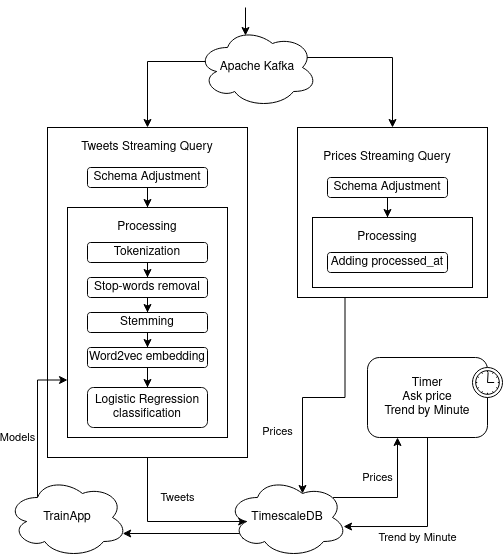
\includegraphics[
		height=10cm,
		keepaspectratio,
    ]{streamapp.png}
    \caption{Schema del funzionamento di StreamApp}
    \label{streamapp}
\end{figure}

\subsection{Training}

Il training dei modelli è svolto per conto della TrainApp: a partire dai tweets
salvati nel database sono stati eseguiti alcuni degli stessi passaggi necessari per
l'analisi in streaming, quali:

\begin{enumerate}
    \item Tokenizzazione.
    \item Rimozione delle stop-words.
    \item Stemming.
\end{enumerate}

Per poi utilizzare i token rimasti per il training del modello Word2Vec, ed in seguito
impiegare la
rappresentazione Word2Vec, come input, insieme all'andamento del prezzo di ask al minuto,
come target,
per allenare il modello di Regressione logistica.

\subsection{Performance del modello}

La TrainApp stessa prima della creazione del modello finale utilizzando la totalità dei dati
ne esegue una validazione dividendo il dataset in trainset e testset e computando il valore AUC
(Area Under ROC).
Purtroppo i risultati ottenuti non sono dei migliori: i valori di AUC sono intorno a 0.5, cioè
le performance sono paragonabili a una scelta random.

Ciò può significare che il contenuto dei tweets generalmente non è correlato all'andamento
del prezzo di ask.
Potrebbe perciò rivelarsi utile un
filtraggio manuale di un insieme ristretto di tweets in modo da selezionare solo quelli rilevanti.

In aggiunta un'ulteriore operazione manuale di etichettatura potrebbe chiarire se l'andamento
dei prezzi sia un parametro adeguato a definire la polarità dei tweets.
\section{Risultati}

Per dimostrare la scalabilità orizzantale dell'applicazione sono state utilizzate le seguenti
macchine:

\begin{enumerate}
    \item un laptop con Intel core i5 e 8gb ram,
    \item un laptop con Intel core i7 e 16gb ram
\end{enumerate}

La maggior parte dei servizi necessari all'applicazione sono stati eseguiti sulla prima macchina:
TimescaleDB, Kafka e Zookeeper, i producer, l'istanza master di Spark, alcune istanze worker ed
infine il processo submit di Spark che "invia" la StreamApp al cluster attraverso il master.

Nella seconda macchina sono stati eseguiti soltanto Spark workers appartenenti allo stesso cluster.

Ogni worker dispone di 1 cpu e 1gb di ram ed il loro numero è stato incrementato gradualmente
allo scopo di testare la scalabilità dell'applicazione in questo modo:

\begin{itemize}
    \item inizialmente (alle 20:50 circa) è stato eseguito un solo worker nella prima macchina
    \item tre minuti dopo ne è stata eseguita un'atra istanza sulla prima macchina
    \item d'ora in poi ogni 3 minuti è stato aggiunto un worker sulla seconda macchina fino a
          a raggiungere un totale di 10 worker sulla seconda macchina più 2 sulla prima
    \item infine sono stati aggiunti altri 4 worker sulla seconda macchina sempre ad intervalli di
          tre minuti.
\end{itemize}

\begin{figure}
    \centering
    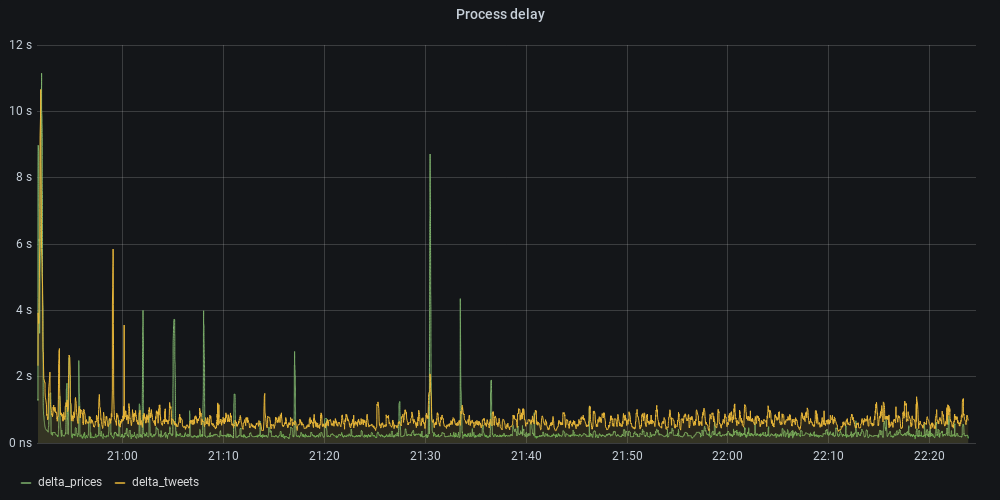
\includegraphics[
		height=5cm,
		keepaspectratio,
    ]{process_delay.png}
    \caption{Process delay}
    \label{processdelay}
\end{figure}

Nella Figura \ref{processdelay} è riportato il grafico che mostra il ritardo nell'analisi dei tweets
e dei prezzi ricevuti calcolato come differenza tra il momento di ricezione (aggiunto dai producer)
ed il momento subito precedente all'inserimento nel database (il ritardo è una media sulle 90 righe
precedente in modo da semplificarne la comprensione).

Si può notare come all'aumentare del numero dei worker il ritardo diminuisce leggermente e
soprattutto come diminuisce il numero e la frequenza dei "picchi".


%\include capitolo risultati/script prodotti
%\include conclusioni

%%aggiungere un capitolo con i software prodotti??? e magari qualcosa sui test??

\bibliography{Report}
\bibliographystyle{ieeetr}

%\nocite{*}

\end{document}